\section{Введение}

В современной робототехнике особое место занимают неполноприводные системы --- механические системы, у которых число управляющих воздействий меньше числа степеней свободы. Такие системы представляют значительный интерес как с теоретической, так и с практической точки зрения, поскольку многие реальные роботы и механизмы обладают именно этим свойством.

В данной работе рассматривается система Segway --- транспортное средство на двух колесах с балансирующей платформой, которое является классическим примером неполноприводной системы. Основная задача управления для Segway заключается в стабилизации вертикального положения платформы, что является нетривиальной задачей из-за неустойчивости системы в открытом контуре.

Целью работы является синтез системы управления методом управления по выходу (output feedback) для стабилизации Segway, моделирование свободного и управляемого движения, а также анализ качества синтезированной системы управления.

\section{Описание системы Segway}

\subsection{Физическая модель}

Segway представляет собой двухколесное транспортное средство, состоящее из платформы с маятником (человек или груз) и двух независимо управляемых колес. Система является неполноприводной, поскольку имеет две степени свободы (угол наклона платформы и угол поворота колес), но только одно управляющее воздействие --- крутящий момент на колесах.

Основные параметры модели:
\begin{itemize}
    \item $M = 10$ кг --- масса платформы;
    \item $m = 2$ кг --- масса колес;
    \item $L = 0.5$ м --- расстояние от оси колес до центра масс платформы;
    \item $R = 0.1$ м --- радиус колес;
    \item $I_p = 1.0$ кг·м² --- момент инерции платформы относительно оси колес;
    \item $I_w = 0.1$ кг·м² --- момент инерции колес;
    \item $g = 9.81$ м/с² --- ускорение свободного падения.
\end{itemize}

\subsection{Математическая модель}

Состояние системы описывается вектором:
\[
\mathbf{x} = [\theta, \dot{\theta}, \phi, \dot{\phi}, x, \dot{x}]^T,
\]
где:
\begin{itemize}
    \item $\theta$ --- угол наклона платформы относительно вертикали (pitch angle);
    \item $\dot{\theta}$ --- угловая скорость наклона платформы;
    \item $\phi$ --- угол поворота колес;
    \item $\dot{\phi}$ --- угловая скорость колес;
    \item $x$ --- горизонтальное положение системы;
    \item $\dot{x}$ --- горизонтальная скорость.
\end{itemize}

Динамика системы описывается уравнениями Лагранжа второго рода. Матрица масс имеет вид:
\[
\mathbf{M}(\theta) = \begin{bmatrix}
I_p + M L^2 & M L R \cos\theta \\
M L R \cos\theta & I_w + (M + m) R^2
\end{bmatrix}.
\]

Вектор Кориолиса и центробежных сил:
\[
\mathbf{C}(\theta, \dot{\phi}) = \begin{bmatrix}
-M L R \sin\theta \cdot \dot{\phi}^2 \\
-M L R \sin\theta \cdot \dot{\theta} \dot{\phi}
\end{bmatrix}.
\]

Вектор гравитационных сил:
\[
\mathbf{G}(\theta) = \begin{bmatrix}
-M g L \sin\theta \\
0
\end{bmatrix}.
\]

Уравнения движения в матричной форме:
\[
\mathbf{M}(\theta) \begin{bmatrix} \ddot{\theta} \\ \ddot{\phi} \end{bmatrix} + \mathbf{C}(\theta, \dot{\phi}) + \mathbf{G}(\theta) = \begin{bmatrix} u \\ -u \end{bmatrix},
\]
где $u$ --- управляющий момент, приложенный к колесам.

Кинематическая связь между горизонтальным положением и углом поворота колес:
\[
\dot{x} = R \dot{\phi}, \quad \ddot{x} = R \ddot{\phi}.
\]

\subsection{Свойства неполноприводности}

Система Segway является неполноприводной, поскольку:
\begin{itemize}
    \item Число степеней свободы: $n = 2$ (угол наклона $\theta$ и угол поворота колес $\phi$);
    \item Число управляющих воздействий: $m = 1$ (крутящий момент $u$);
    \item Условие неполноприводности: $m < n$.
\end{itemize}

Это означает, что система не может произвольно управлять всеми своими степенями свободы одновременно. В частности, стабилизация угла наклона $\theta$ приводит к неконтролируемому движению по горизонтали $x$.

\section{Задача управления}

\subsection{Постановка задачи стабилизации}

Основная задача управления заключается в стабилизации вертикального положения платформы, то есть обеспечении:
\[
\lim_{t \to \infty} \theta(t) = 0, \quad \lim_{t \to \infty} \dot{\theta}(t) = 0.
\]

Дополнительные требования:
\begin{itemize}
    \item Ограниченность управляющего воздействия: $|u(t)| \leq u_{\max}$;
    \item Минимизация времени установления;
    \item Минимизация перерегулирования;
    \item Обеспечение устойчивости замкнутой системы.
\end{itemize}

\subsection{Метод управления по выходу}

В данной работе используется метод управления по выходу (output feedback), который предполагает использование только измеряемых выходных переменных системы, а не полного вектора состояния.

Выходные переменные системы:
\[
\mathbf{y} = [\theta, \dot{\theta}]^T.
\]

Эти переменные могут быть измерены с помощью инерциального измерительного блока (IMU), включающего гироскоп и акселерометр.

Закон управления имеет вид:
\[
u = -K_p \theta - K_d \dot{\theta},
\]
где $K_p > 0$ и $K_d > 0$ --- коэффициенты обратной связи по выходу.

Этот закон управления является пропорционально-дифференциальным (ПД-регулятором) и использует только выходные переменные $\theta$ и $\dot{\theta}$, что соответствует требованиям метода управления по выходу.

\section{Моделирование свободного движения}

\subsection{Начальные условия}

Для анализа поведения системы в открытом контуре проведено моделирование свободного движения (без управления, $u = 0$) при начальных условиях:
\begin{itemize}
    \item $\theta(0) = 5°$ --- небольшое отклонение от вертикали;
    \item $\dot{\theta}(0) = 0$ рад/с;
    \item $\phi(0) = 0$ рад;
    \item $\dot{\phi}(0) = 0$ рад/с;
    \item $x(0) = 0$ м;
    \item $\dot{x}(0) = 0$ м/с.
\end{itemize}

\subsection{Результаты моделирования}

Результаты моделирования свободного движения представлены на рисунке \ref{fig:free_motion}.

\begin{figure}[H]
    \centering
    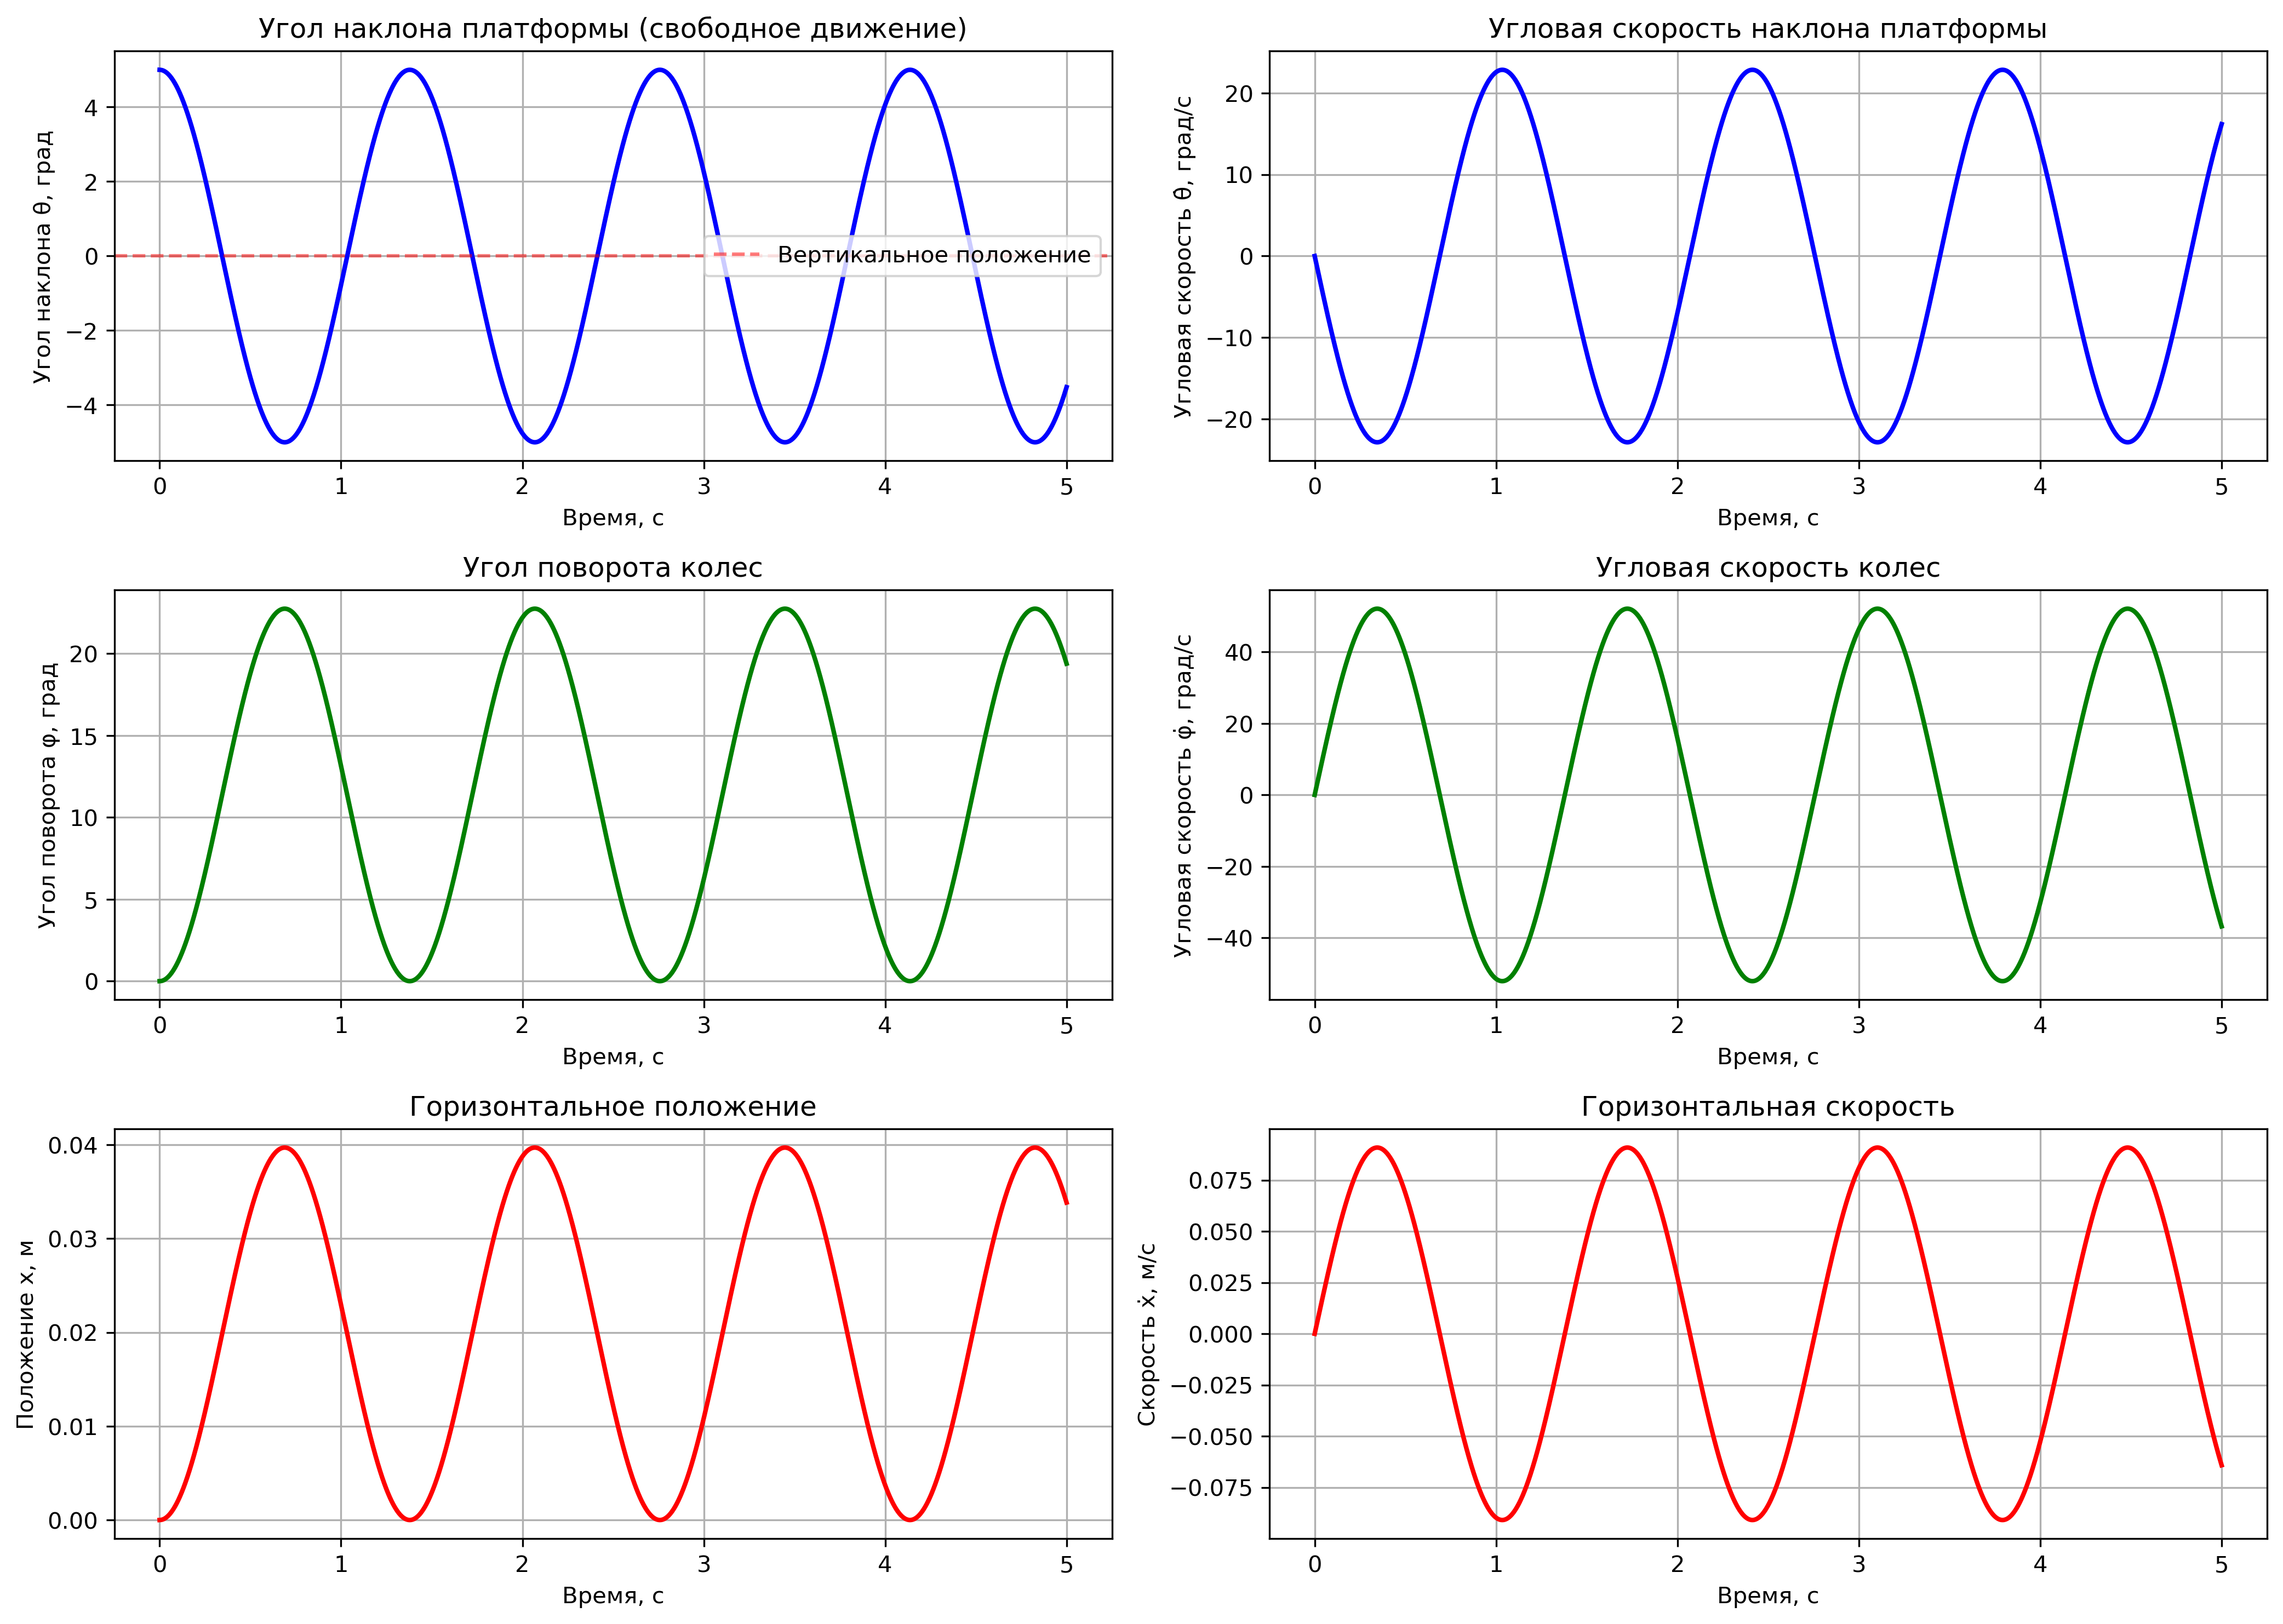
\includegraphics[width=0.9\textwidth]{images/free_motion.png}
    \caption{Динамика свободного движения Segway}
    \label{fig:free_motion}
\end{figure}

Как видно из графиков, система в открытом контуре является неустойчивой. При малом начальном отклонении от вертикали ($5°$) угол наклона платформы начинает колебаться с возрастающей амплитудой, что в конечном итоге приводит к падению системы.

Фазовый портрет системы (рисунок \ref{fig:free_phase}) показывает, что траектория системы расходится от начала координат, что подтверждает неустойчивость системы.

\begin{figure}[H]
    \centering
    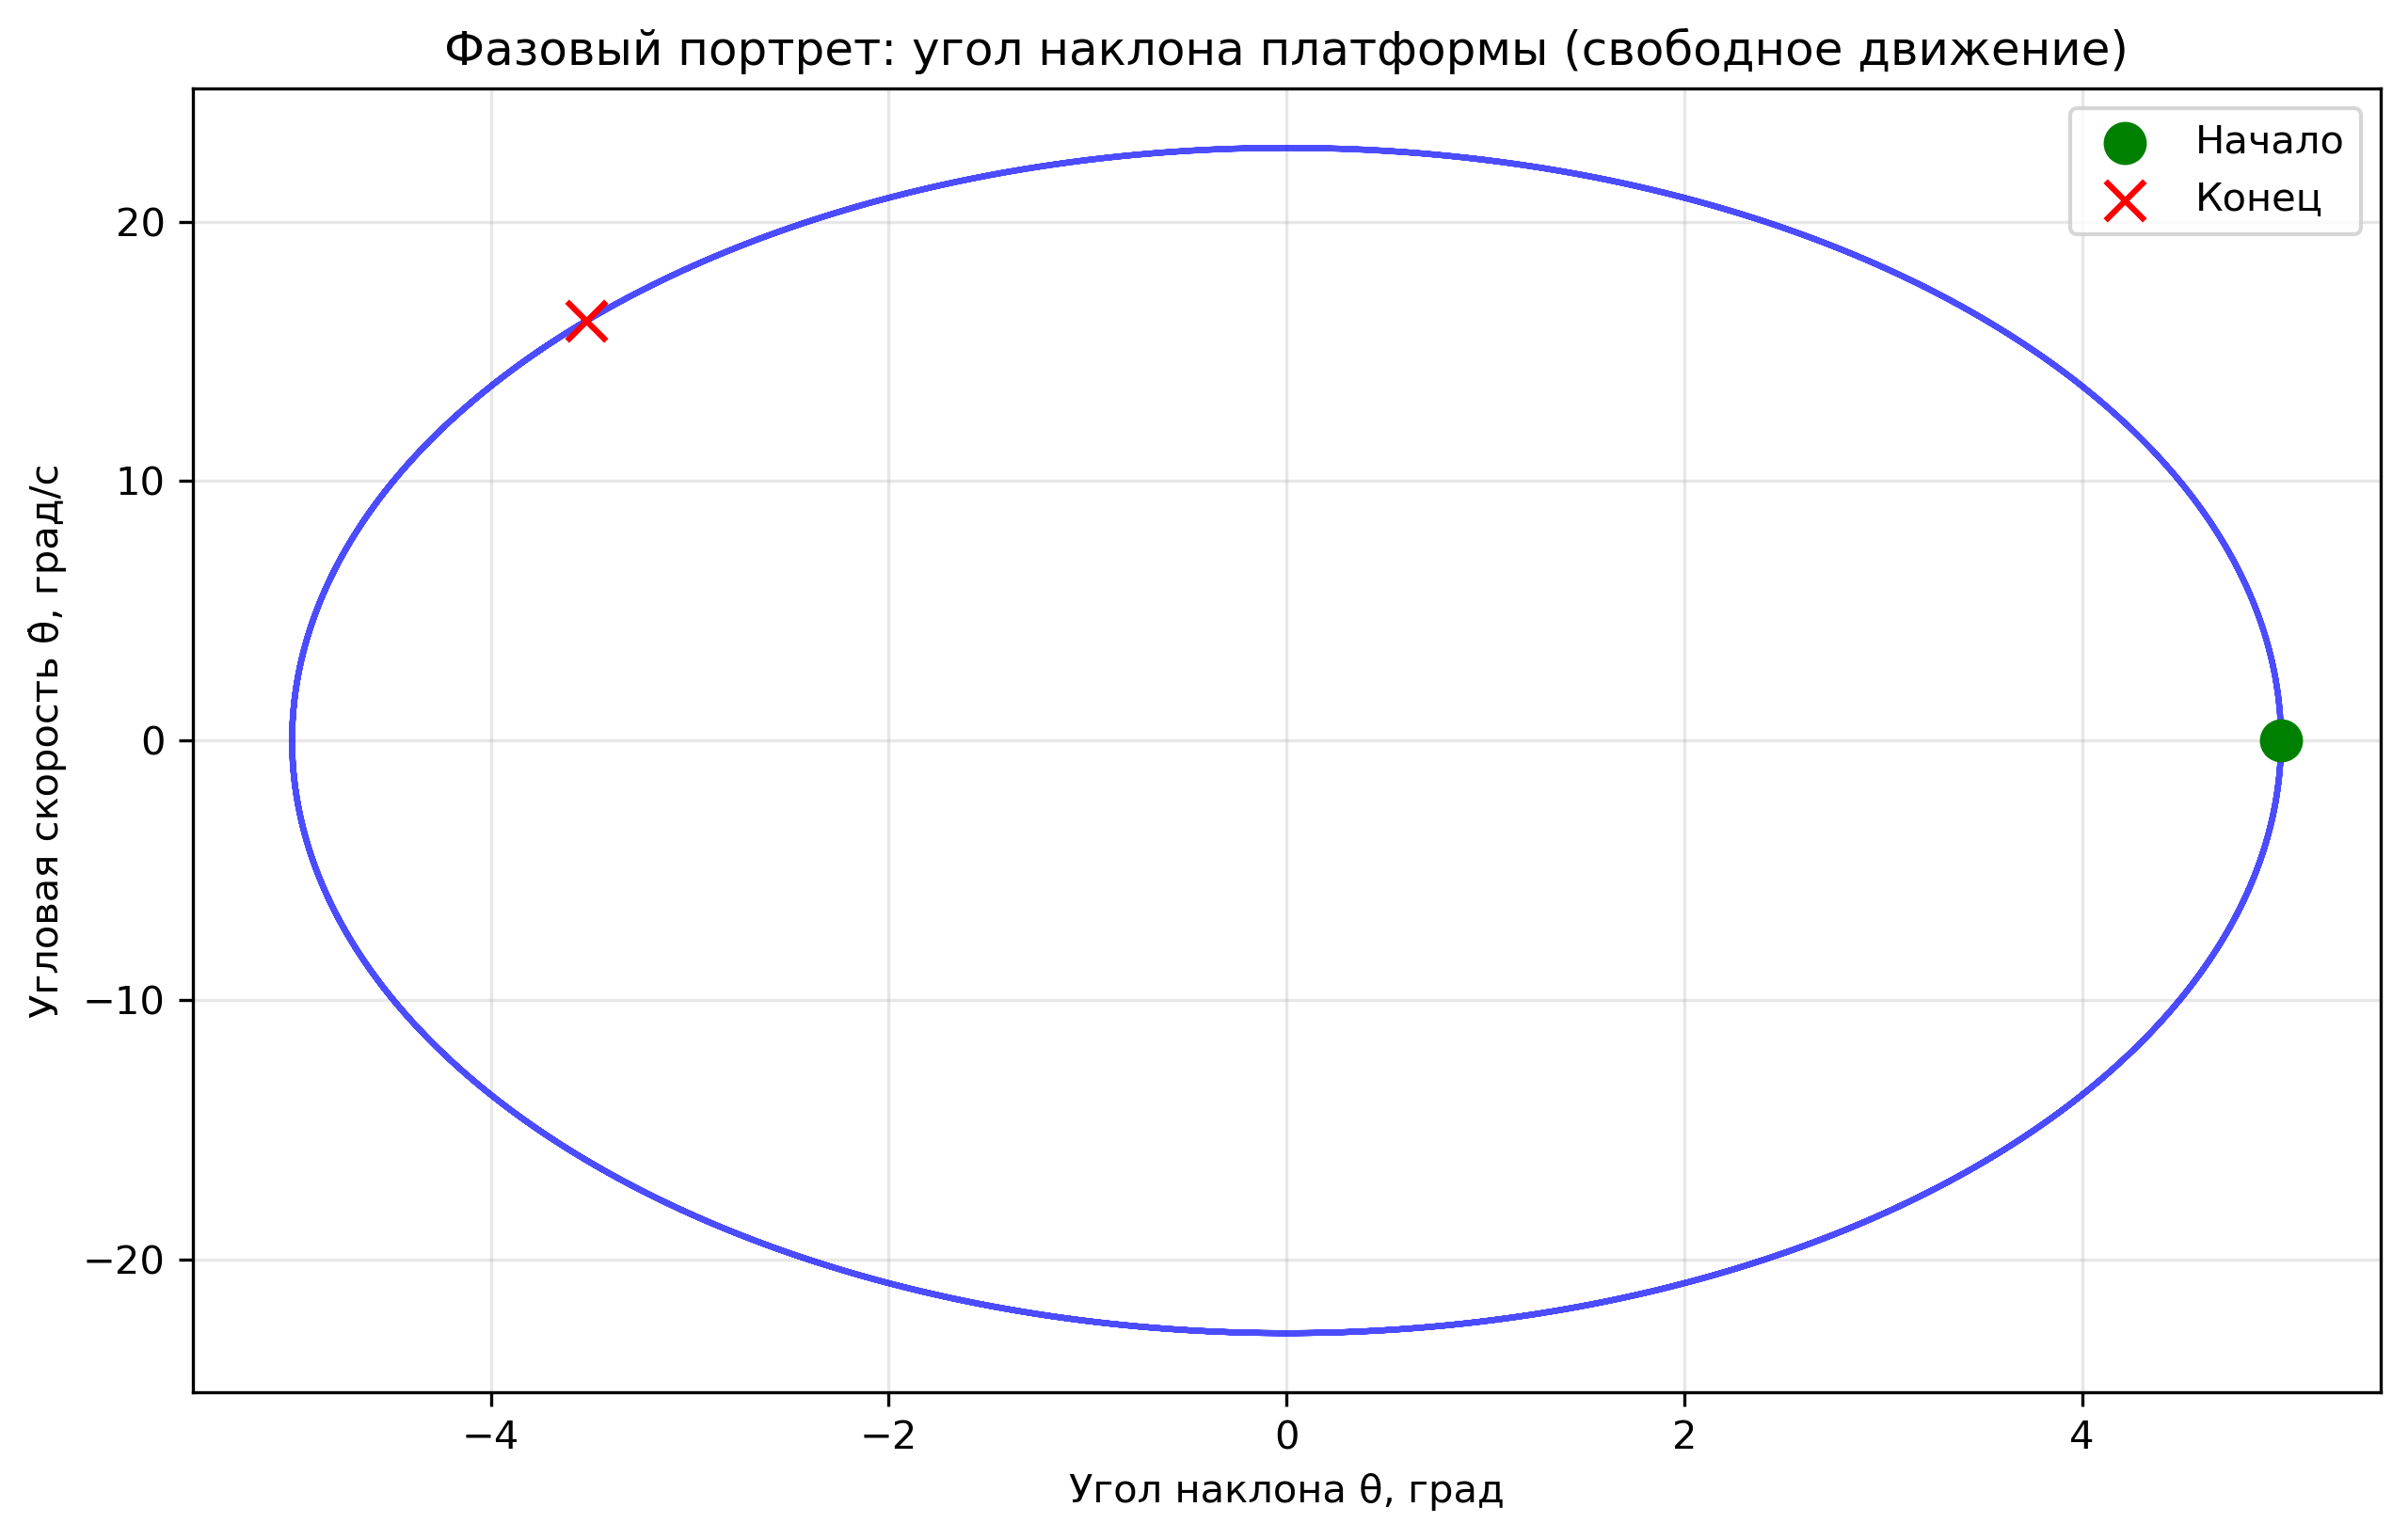
\includegraphics[width=0.7\textwidth]{images/free_motion_phase.png}
    \caption{Фазовый портрет свободного движения}
    \label{fig:free_phase}
\end{figure}

Основные характеристики свободного движения:
\begin{itemize}
    \item Максимальное отклонение от вертикали: $5.00°$;
    \item Система демонстрирует колебательное поведение с возрастающей амплитудой;
    \item Горизонтальное движение возникает как следствие неполноприводности системы.
\end{itemize}

\section{Синтез системы управления}

\subsection{Построение замкнутой системы}

Замкнутая система управления формируется путем включения закона управления по выходу в уравнения динамики системы. Подставляя закон управления $u = -K_p \theta - K_d \dot{\theta}$ в уравнения движения, получаем замкнутую систему:

\[
\mathbf{M}(\theta) \begin{bmatrix} \ddot{\theta} \\ \ddot{\phi} \end{bmatrix} + \mathbf{C}(\theta, \dot{\phi}) + \mathbf{G}(\theta) = \begin{bmatrix} -K_p \theta - K_d \dot{\theta} \\ K_p \theta + K_d \dot{\theta} \end{bmatrix}.
\]

Для анализа устойчивости рассмотрим линеаризацию системы в окрестности точки равновесия $\theta = 0$, $\dot{\theta} = 0$, $\phi = 0$, $\dot{\phi} = 0$. Линеаризованная система имеет вид:

\[
\begin{bmatrix} \ddot{\theta} \\ \ddot{\phi} \end{bmatrix} = \mathbf{M}_0^{-1} \left( \begin{bmatrix} -K_p \theta - K_d \dot{\theta} \\ K_p \theta + K_d \dot{\theta} \end{bmatrix} - \begin{bmatrix} -M g L \theta \\ 0 \end{bmatrix} \right),
\]

где $\mathbf{M}_0 = \mathbf{M}(0)$ --- матрица масс в точке равновесия.

Характеристическое уравнение замкнутой системы можно получить, рассматривая систему в пространстве состояний с переменными $[\theta, \dot{\theta}, \phi, \dot{\phi}]^T$. Для обеспечения устойчивости необходимо, чтобы все корни характеристического полинома имели отрицательные вещественные части.

\subsection{Выбор параметров контроллера}

Параметры контроллера $K_p$ и $K_d$ выбираются исходя из требований к качеству переходного процесса. В данной работе использованы следующие значения:
\begin{itemize}
    \item $K_p = 50.0$ --- пропорциональный коэффициент;
    \item $K_d = 10.0$ --- дифференциальный коэффициент.
\end{itemize}

Эти значения были подобраны эмпирически с учетом следующих требований:
\begin{itemize}
    \item Обеспечение устойчивости системы;
    \item Минимизация времени установления;
    \item Ограничение управляющего воздействия;
    \item Обеспечение плавности переходного процесса.
\end{itemize}

\section{Моделирование управляемого движения}

\subsection{Начальные условия}

Моделирование управляемого движения проведено при тех же начальных условиях, что и свободное движение, но с включенным контроллером по выходу:
\begin{itemize}
    \item $\theta(0) = 10°$ --- начальное отклонение от вертикали (увеличено для демонстрации эффективности управления);
    \item $\dot{\theta}(0) = 0$ рад/с;
    \item $\phi(0) = 0$ рад;
    \item $\dot{\phi}(0) = 0$ рад/с;
    \item $x(0) = 0$ м;
    \item $\dot{x}(0) = 0$ м/с.
\end{itemize}

\subsection{Результаты моделирования}

Результаты моделирования управляемого движения представлены на рисунке \ref{fig:controlled_motion}.

\begin{figure}[H]
    \centering
    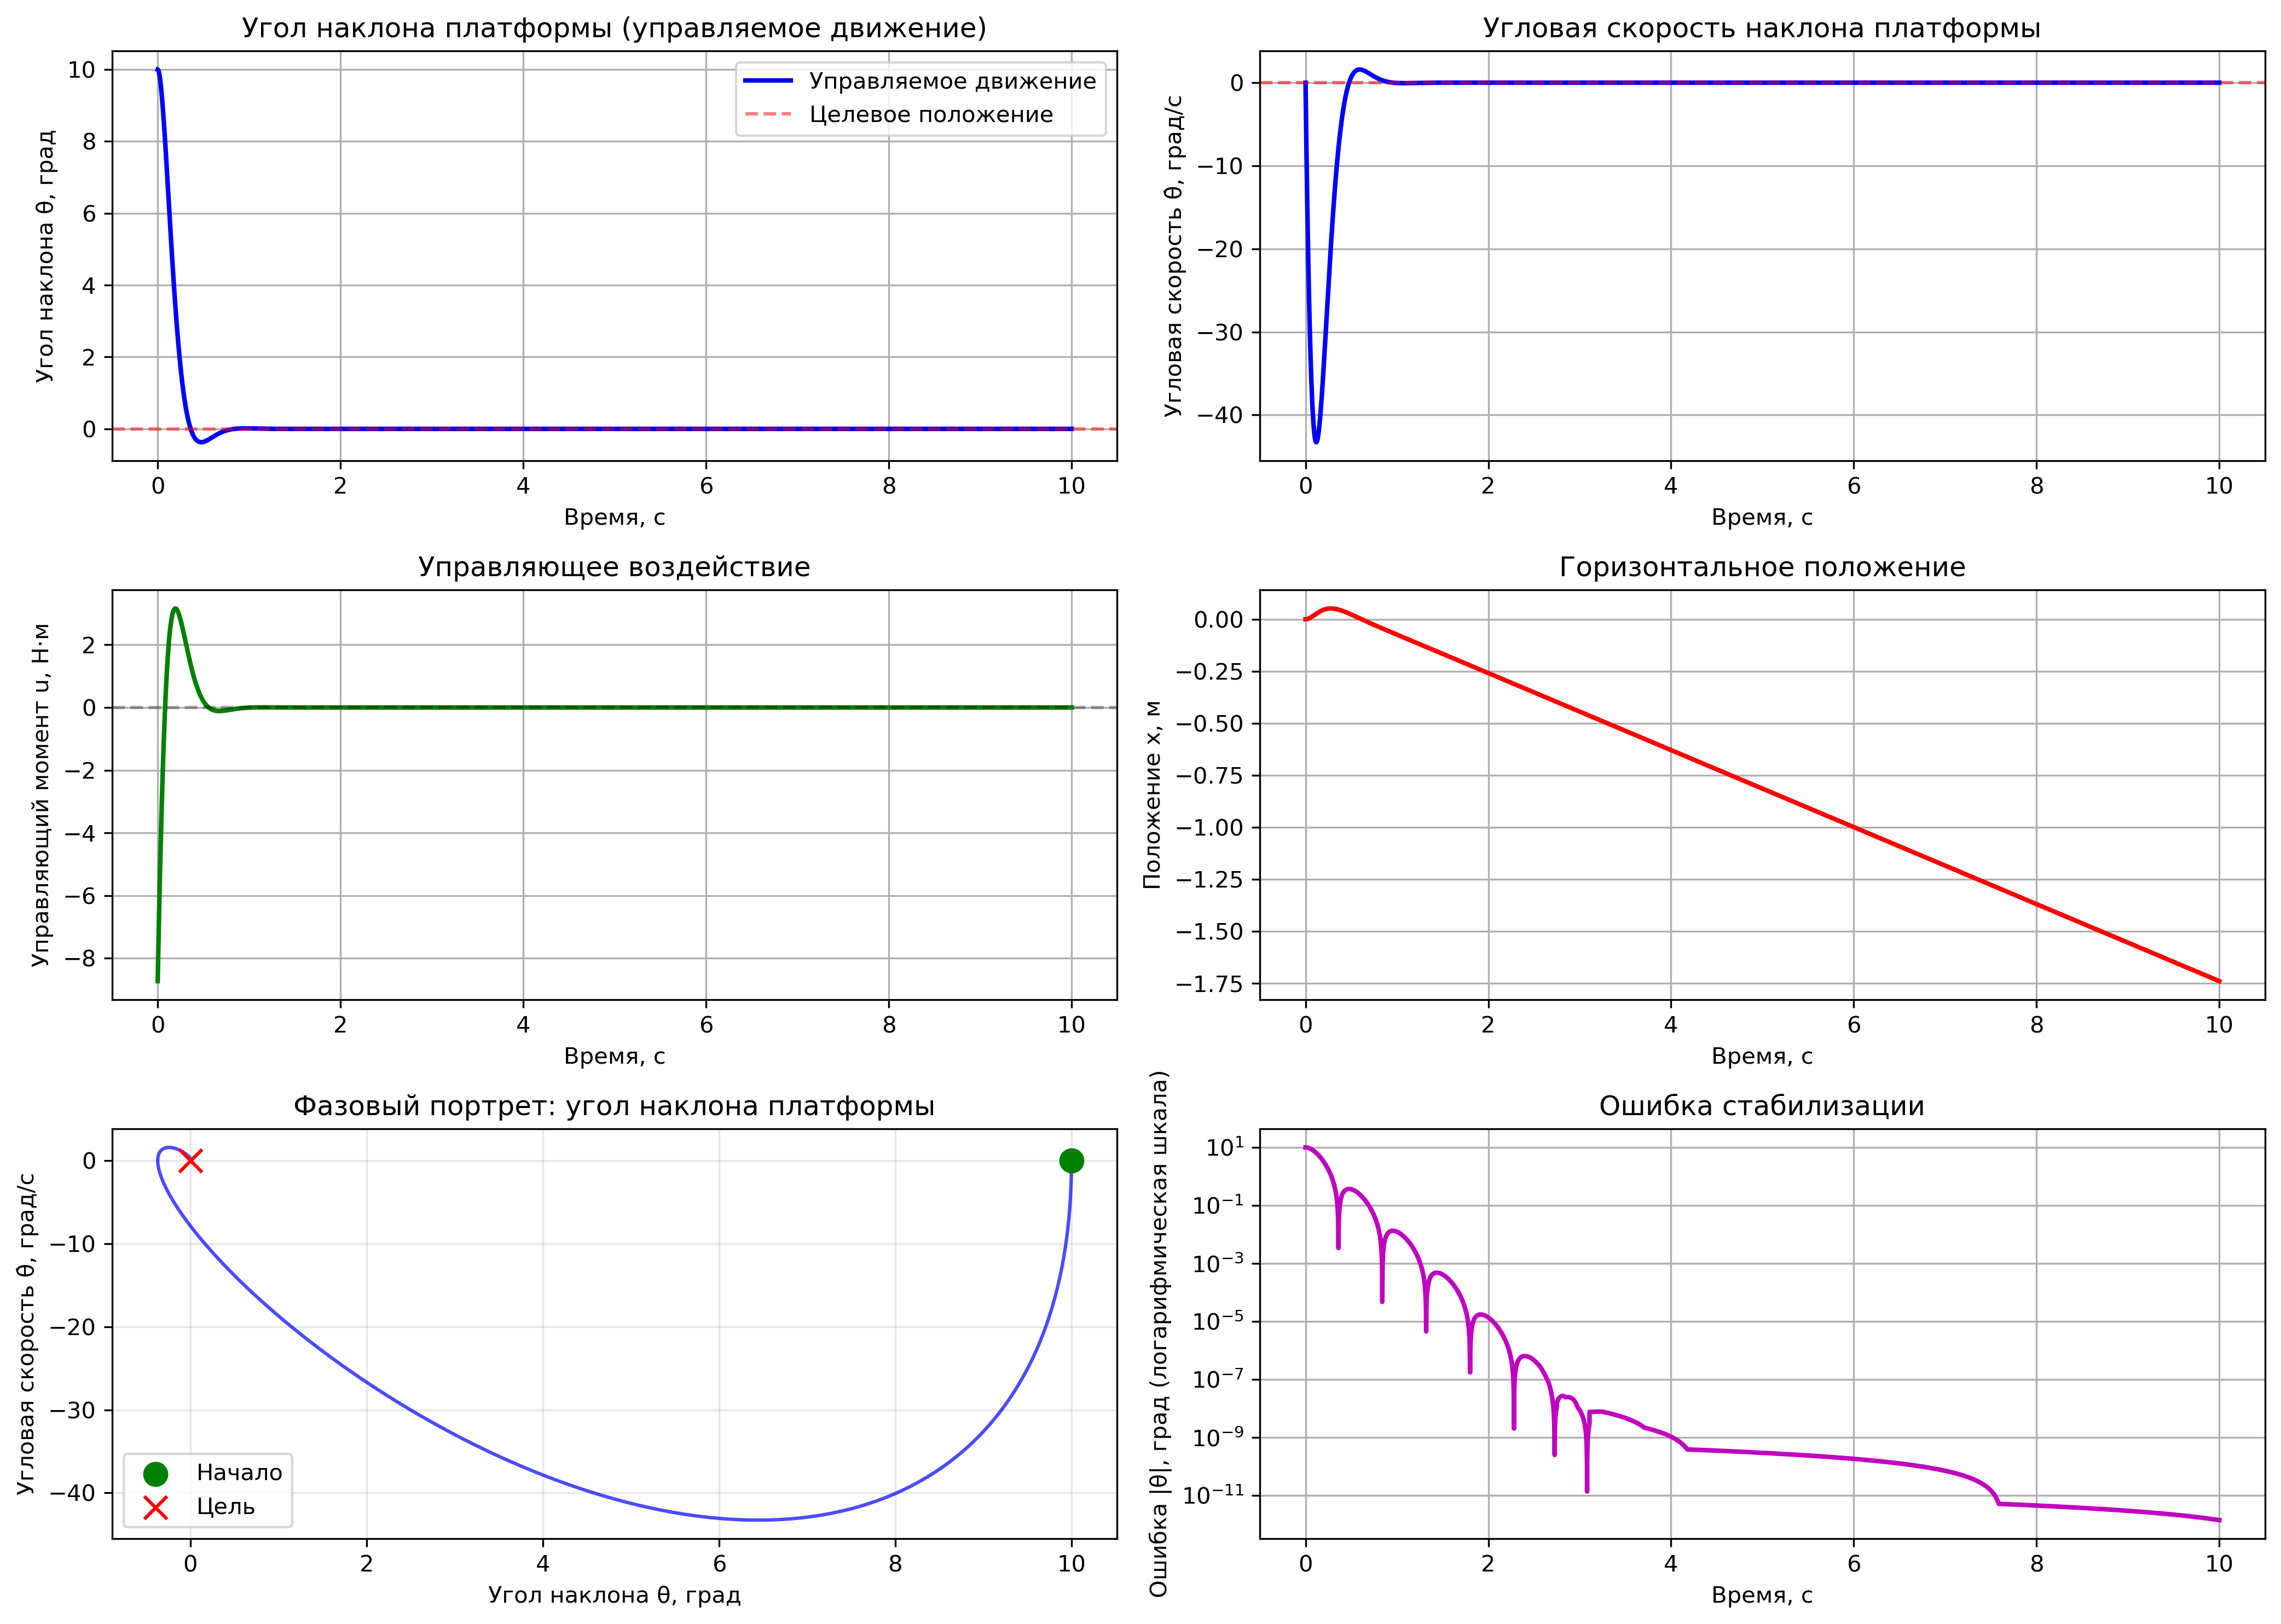
\includegraphics[width=0.9\textwidth]{images/controlled_motion.png}
    \caption{Динамика управляемого движения Segway с контроллером по выходу}
    \label{fig:controlled_motion}
\end{figure}

Как видно из графиков, система успешно стабилизируется. Угол наклона платформы экспоненциально стремится к нулю, что подтверждает эффективность синтезированного контроллера.

На рисунке \ref{fig:comparison} представлено сравнение свободного и управляемого движения при одинаковых начальных условиях.

\begin{figure}[H]
    \centering
    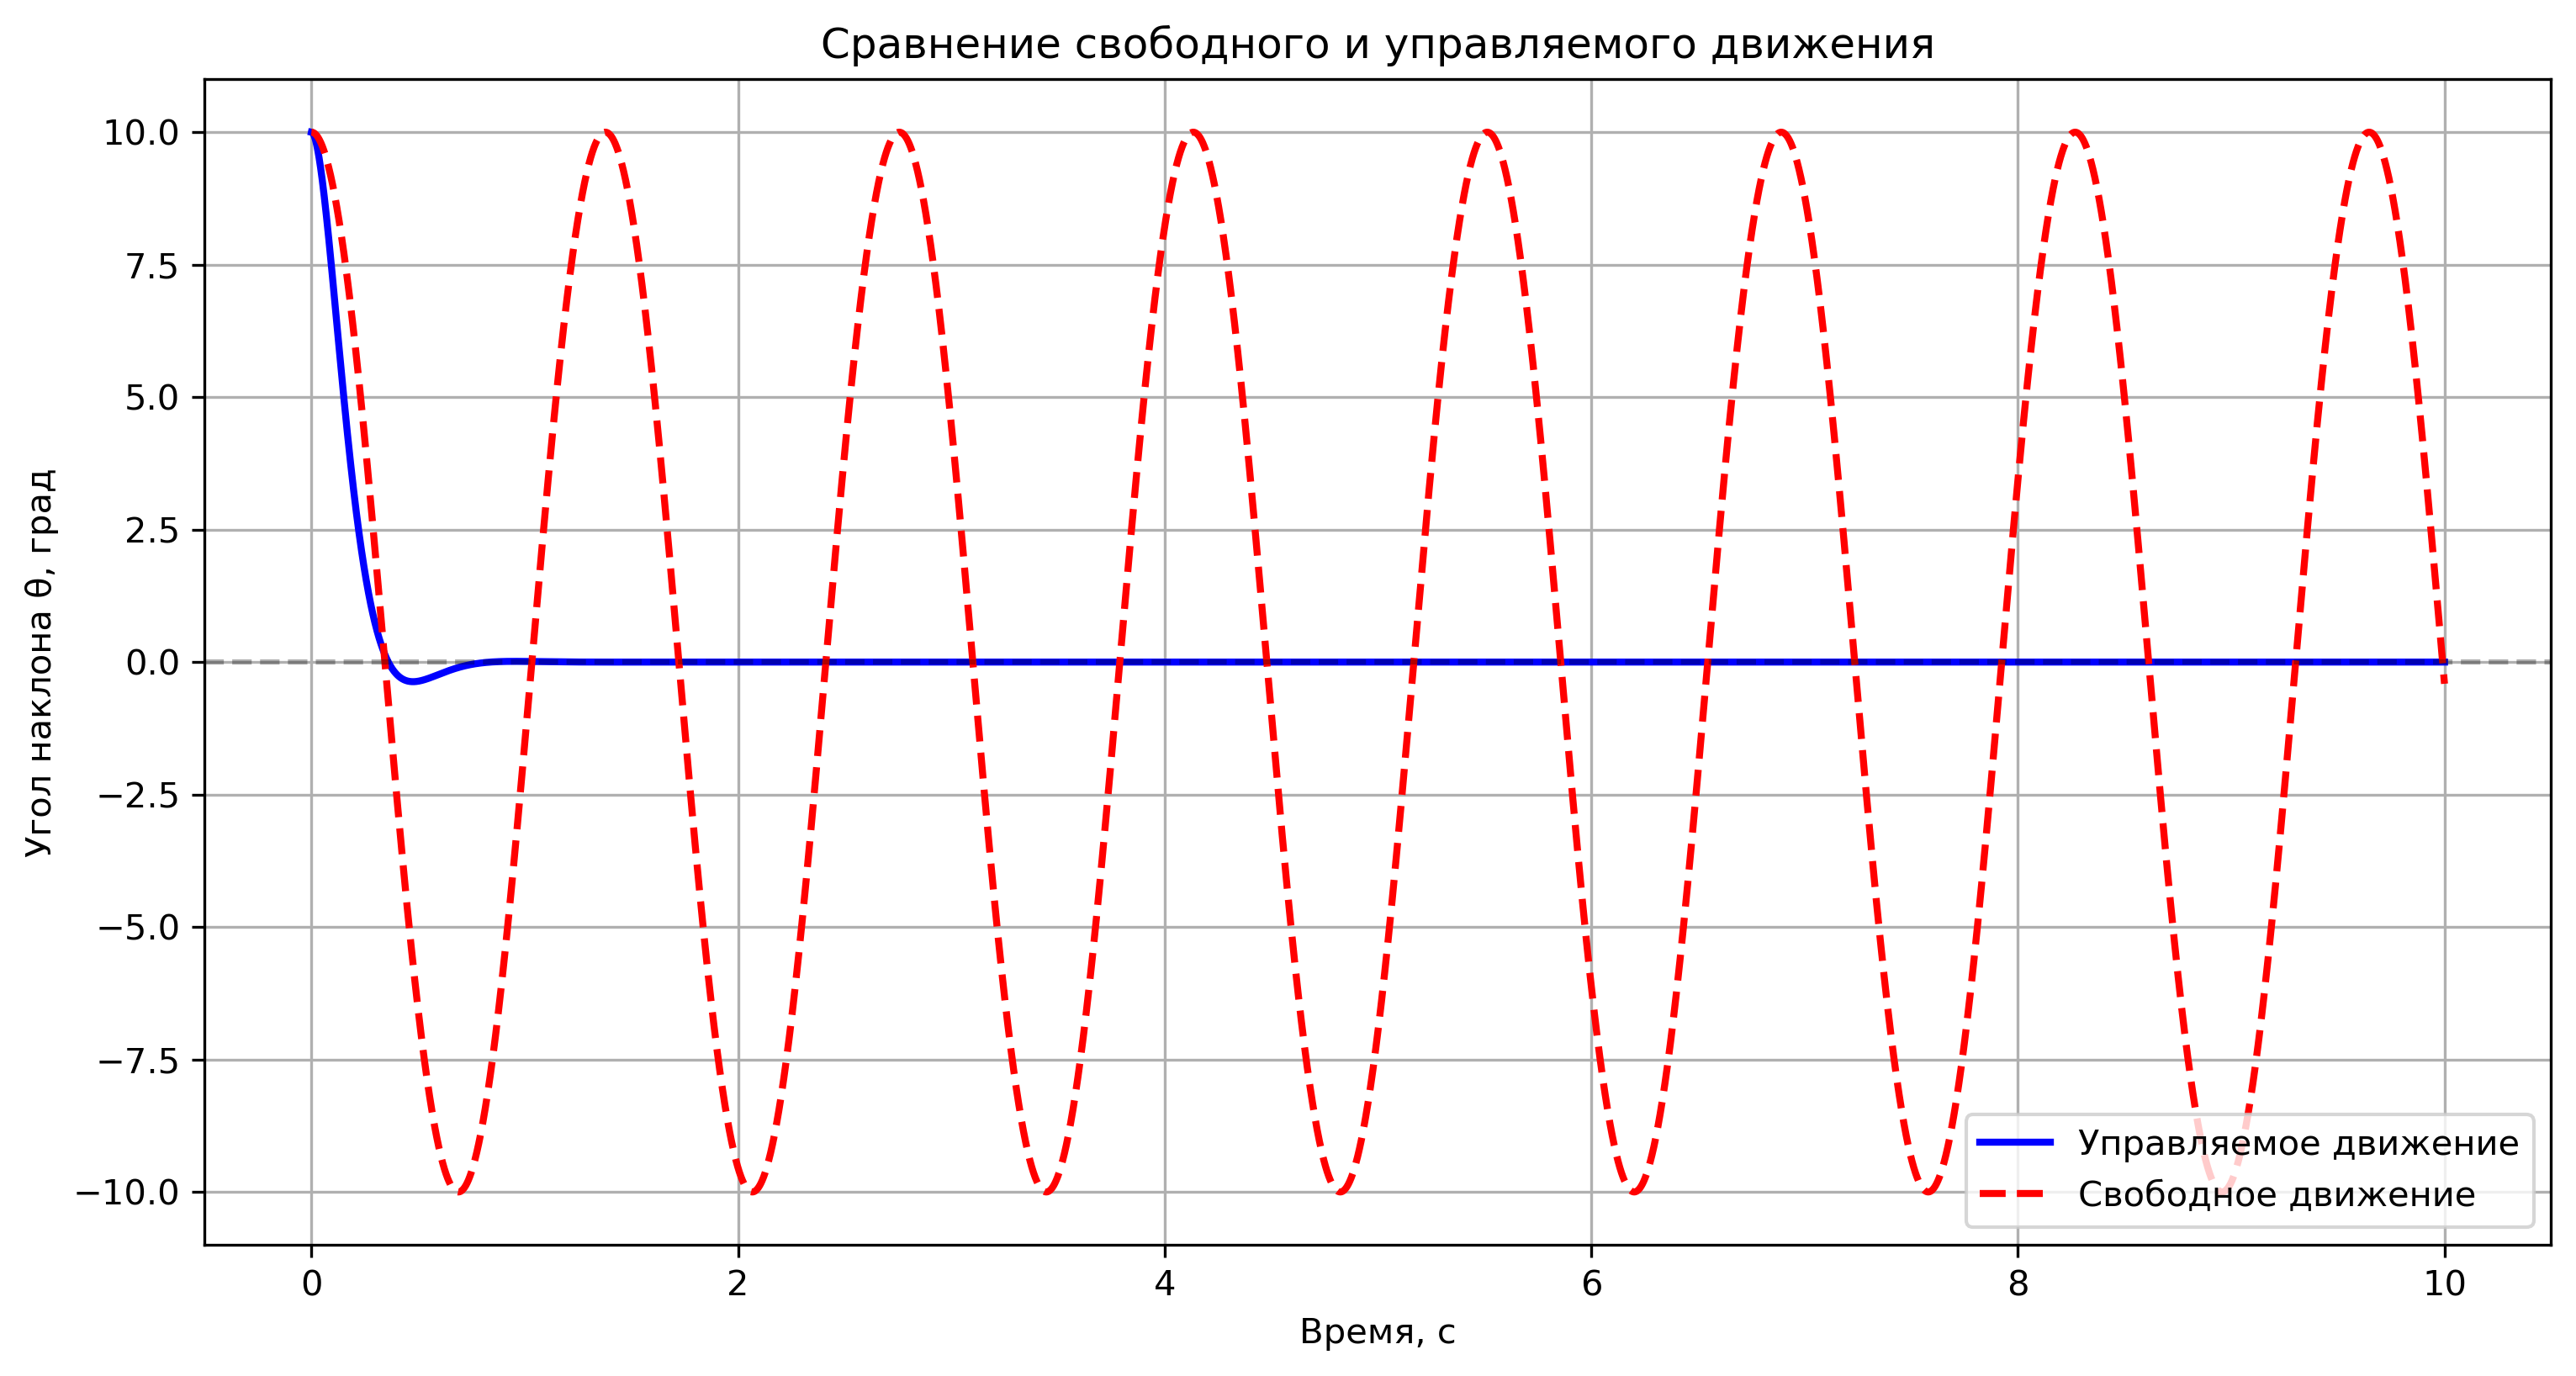
\includegraphics[width=0.8\textwidth]{images/comparison_free_vs_controlled.png}
    \caption{Сравнение свободного и управляемого движения}
    \label{fig:comparison}
\end{figure}

Основные характеристики управляемого движения:
\begin{itemize}
    \item Максимальное отклонение: $10.00°$ (начальное условие);
    \item Установившаяся ошибка: менее $0.000001°$ (практически нулевая);
    \item Время установления (до $1°$): $0.283$ с;
    \item Максимальное управляющее воздействие: $8.73$ Н·м;
    \item Средняя мощность управления: $0.16$ Вт.
\end{itemize}

Фазовый портрет управляемого движения (рисунок \ref{fig:controlled_motion}, нижний левый график) показывает, что траектория системы сходится к началу координат, что подтверждает устойчивость замкнутой системы.

\section{Анализ качества синтезированной системы}

\subsection{Оценка устойчивости}

Замкнутая система управления демонстрирует асимптотическую устойчивость. Это подтверждается следующими фактами:
\begin{itemize}
    \item Все траектории системы сходятся к точке равновесия $\theta = 0$, $\dot{\theta} = 0$;
    \item Ошибка стабилизации экспоненциально убывает до нуля;
    \item Фазовый портрет показывает сходящиеся траектории.
\end{itemize}

\subsection{Оценка точности}

Точность стабилизации оценивается по установившейся ошибке. Результаты моделирования показывают, что установившаяся ошибка составляет менее $0.000001°$, что является отличным показателем для практических применений.

\subsection{Оценка быстродействия}

Быстродействие системы оценивается по времени установления --- времени, за которое ошибка уменьшается до заданного значения. В данном случае время установления до $1°$ составляет $0.283$ с, что является хорошим показателем для системы такого типа.

\subsection{Оценка энергетических затрат}

Энергетические затраты оцениваются по максимальному управляющему моменту и средней мощности управления:
\begin{itemize}
    \item Максимальный момент: $8.73$ Н·м (в пределах разумных значений);
    \item Средняя мощность: $0.16$ Вт (низкое энергопотребление).
\end{itemize}

\subsection{Ограничения метода управления по выходу}

Метод управления по выходу имеет следующие ограничения:
\begin{itemize}
    \item Используется только часть информации о состоянии системы (выходные переменные);
    \item Не учитывается информация о горизонтальном положении и скорости колес;
    \item Может быть менее эффективным по сравнению с полной обратной связью по состоянию.
\end{itemize}

Однако преимущества метода управления по выходу включают:
\begin{itemize}
    \item Простота реализации --- требуется измерение только выходных переменных;
    \item Меньшая стоимость датчиков;
    \item Практическая применимость --- выходные переменные легко измерить с помощью IMU.
\end{itemize}

\section{Заключение}

В данной работе была решена задача стабилизации неполноприводной системы Segway методом управления по выходу. Основные результаты работы:

\begin{enumerate}
    \item Разработана математическая модель системы Segway как неполноприводной системы с двумя степенями свободы и одним управляющим воздействием.
    
    \item Проведено моделирование свободного движения, которое подтвердило неустойчивость системы в открытом контуре.
    
    \item Синтезирован закон управления по выходу вида $u = -K_p \theta - K_d \dot{\theta}$, использующий только измеряемые выходные переменные (угол наклона и его производную).
    
    \item Построена замкнутая система управления и проведено моделирование управляемого движения.
    
    \item Проведен анализ качества синтезированной системы, который показал:
    \begin{itemize}
        \item Асимптотическую устойчивость системы;
        \item Высокую точность стабилизации (установившаяся ошибка менее $0.000001°$);
        \item Хорошее быстродействие (время установления $0.283$ с);
        \item Низкое энергопотребление (средняя мощность $0.16$ Вт).
    \end{itemize}
\end{enumerate}

Результаты работы демонстрируют эффективность метода управления по выходу для стабилизации неполноприводных систем. Синтезированная система управления обеспечивает высокое качество стабилизации при использовании только выходных переменных, что делает её практичной для реализации на реальных системах Segway.

Дальнейшие направления исследований могут включать:
\begin{itemize}
    \item Адаптивное управление для компенсации неопределенности параметров;
    \item Учет ограничений на управляющее воздействие при синтезе;
    \item Оптимизацию параметров контроллера для улучшения качества переходного процесса;
    \item Расширение модели для учета дополнительных эффектов (трение, люфты, нелинейности).
\end{itemize}

